% 固定来源 PDF 印刷页 84 第 8 题四组选项图象的矢量示意重绘。
% 选项相对形状、抛物线开口/过原点关系和指数曲线过 (0,1) 按原图描绘；曲线比例仅为示意。
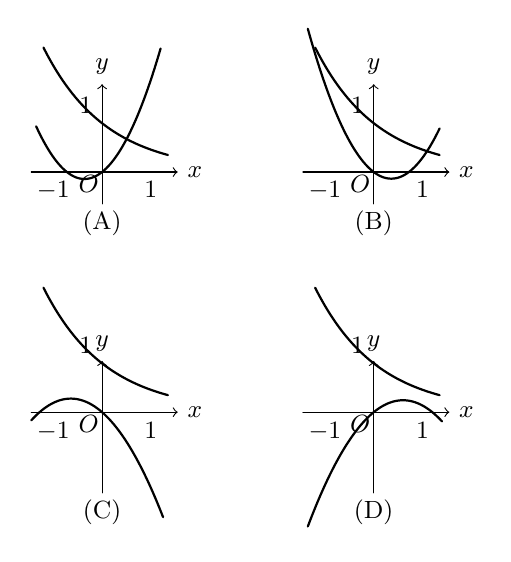
\begin{tikzpicture}[x=.62cm,y=.62cm,font=\small,line cap=round,line join=round]
  % (A) upward parabola with its second zero left of the origin.
  \begin{scope}
    \draw[->] (-1.45,0)--(1.55,0) node[right] {$x$};
    \draw[->] (0,-.65)--(0,1.8) node[above] {$y$};
    \draw[thick,domain=-1.35:1.2,samples=70,variable=\x]
      plot (\x,{1.1*\x*(\x+.72)});
    \draw[thick,domain=-1.2:1.35,samples=70,variable=\x]
      plot (\x,{exp(-.78*\x)});
    \node[below left,inner sep=1pt] at (0,0) {$O$};
    \node[below] at (-1,0) {$-1$}; \node[below] at (1,0) {$1$};
    \node[above left] at (0,1) {$1$}; \node at (0,-1.05) {(A)};
  \end{scope}
  % (B) upward parabola with its second zero right of the origin.
  \begin{scope}[xshift=3.45cm]
    \draw[->] (-1.45,0)--(1.55,0) node[right] {$x$};
    \draw[->] (0,-.65)--(0,1.8) node[above] {$y$};
    \draw[thick,domain=-1.35:1.35,samples=70,variable=\x]
      plot (\x,{1.05*\x*(\x-.72)});
    \draw[thick,domain=-1.2:1.35,samples=70,variable=\x]
      plot (\x,{exp(-.78*\x)});
    \node[below left,inner sep=1pt] at (0,0) {$O$};
    \node[below] at (-1,0) {$-1$}; \node[below] at (1,0) {$1$};
    \node[above left] at (0,1) {$1$}; \node at (0,-1.05) {(B)};
  \end{scope}
  % (C) downward parabola with its second zero left of the origin.
  \begin{scope}[yshift=-3.05cm]
    \draw[->] (-1.45,0)--(1.55,0) node[right] {$x$};
    \draw[->] (0,-1.65)--(0,1.05) node[above] {$y$};
    \draw[thick,domain=-1.45:1.25,samples=70,variable=\x]
      plot (\x,{-.68*\x*(\x+1.28)});
    \draw[thick,domain=-1.2:1.35,samples=70,variable=\x]
      plot (\x,{exp(-.78*\x)});
    \node[below left,inner sep=1pt] at (0,0) {$O$};
    \node[below] at (-1,0) {$-1$}; \node[below] at (1,0) {$1$};
    \node[above left] at (0,1) {$1$}; \node at (0,-2.05) {(C)};
  \end{scope}
  % (D) downward parabola with its second zero right of the origin.
  \begin{scope}[xshift=3.45cm,yshift=-3.05cm]
    \draw[->] (-1.45,0)--(1.55,0) node[right] {$x$};
    \draw[->] (0,-1.65)--(0,1.05) node[above] {$y$};
    \draw[thick,domain=-1.35:1.4,samples=70,variable=\x]
      plot (\x,{-.68*\x*(\x-1.2)});
    \draw[thick,domain=-1.2:1.35,samples=70,variable=\x]
      plot (\x,{exp(-.78*\x)});
    \node[below left,inner sep=1pt] at (0,0) {$O$};
    \node[below] at (-1,0) {$-1$}; \node[below] at (1,0) {$1$};
    \node[above left] at (0,1) {$1$}; \node at (0,-2.05) {(D)};
  \end{scope}
\end{tikzpicture}
